
An attempt was made to find a dataset with handwritten text, but no dataset that fulfilled our requirements was found.
The datasets that were found would require a lot of preprocessing. 
Figure~\ref{figure:wordsexamples} shows a sample from one of the datasets we found.
To get good results from that kind of dataset it would be necessary to implement baseline slant normalization, skew correction, skeleton calculation and so on.

\begin{figure}[h!]
\centering
 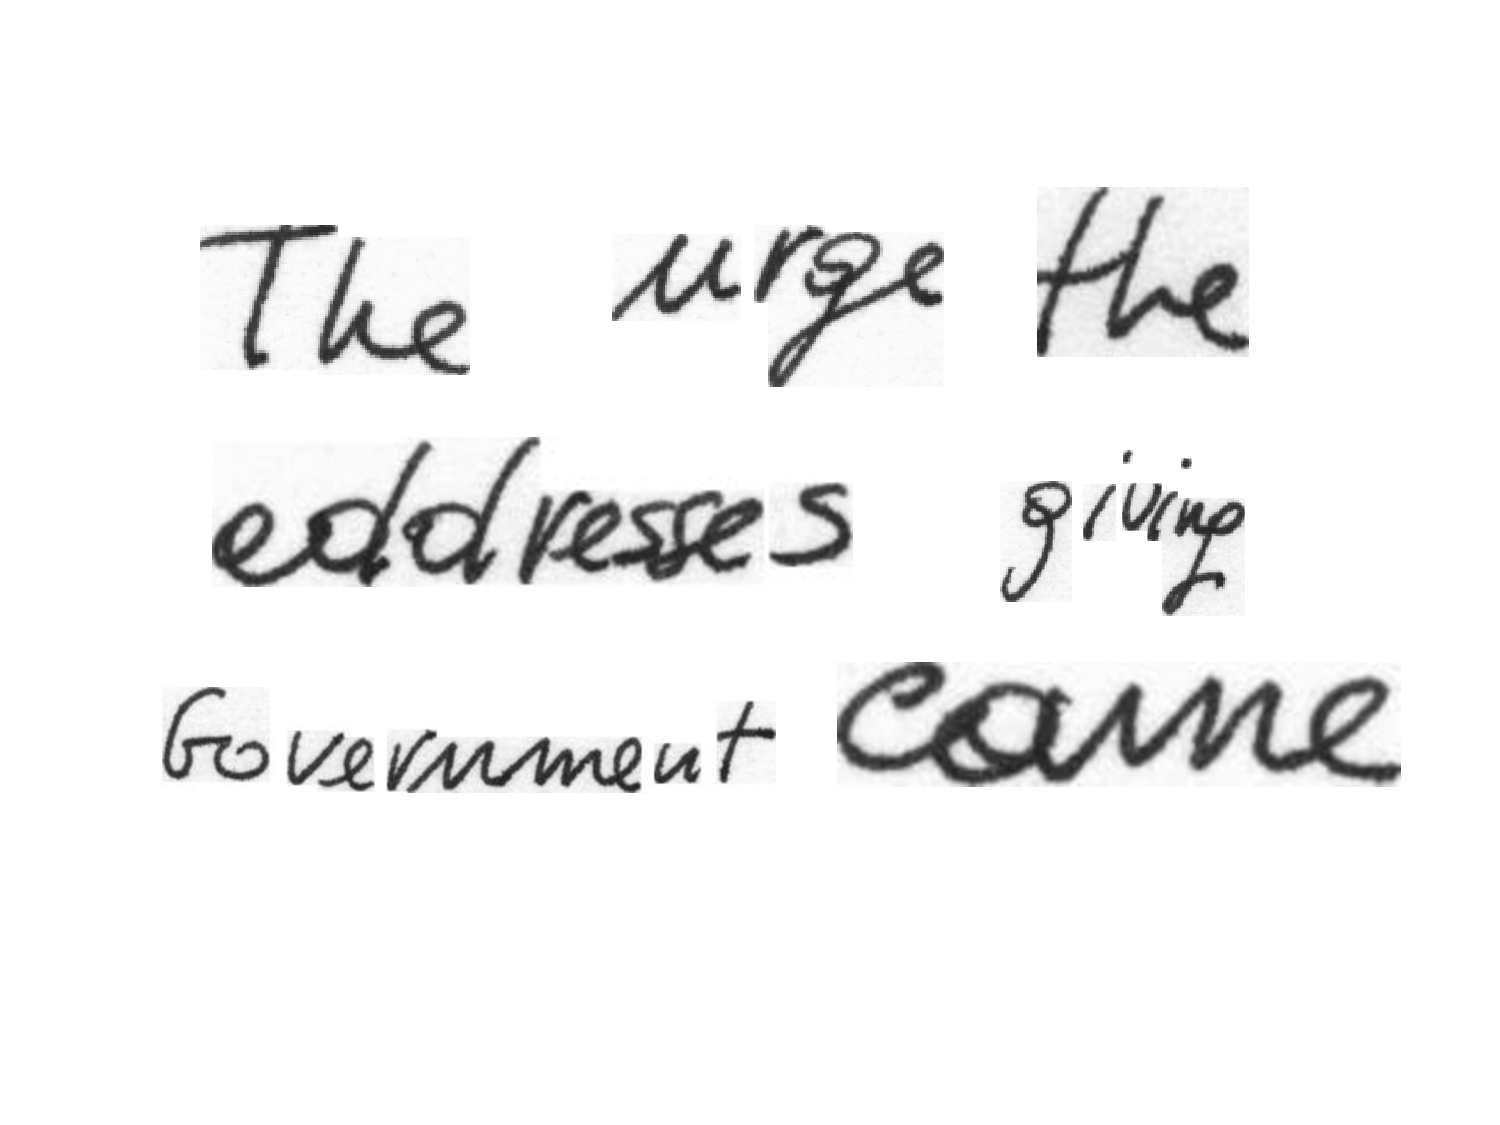
\includegraphics[width=3in]{datasets_examples}
\caption{Word image examples.}
\label{figure:wordsexamples}
\end{figure}

Therefore, instead of spending a lot of time preprocessing word images, we implemented a Graphical User Interface to create our own dataset.
The largest advantages of this solution is that our solution records one pixel wide lines and the characters are already separated. 
A large part of the work, image processing, was thus reduced significantly.
Our dataset contains 100 examples for every capital letter in the Latin alphabet\footnote{The dataset is available together with the source code for the system. See appendix~\ref{app:source_code}.}.
An example image from our character image dataset can be found in Figure~\ref{fig:image_feature_extraction} that shows the feature extraction process.

To get a dataset for training the word classifier a generator was created\footnote{Please, see HandReco\/src\/api\/word\_examples\_generator.py in the source code for documentation of the word example generator. See appendix~\ref{app:source_code}.}.
The generator creates random errors in the words given as input.
To generate the dataset is obviously not optimal for practical applications, but it is good enough to test the implementation.
